\documentclass{article}

\usepackage[margin=1in]{geometry}
\usepackage{amsmath,amsthm,amssymb}
\usepackage{bbm,enumerate,mathtools}
\usepackage[hidelinks]{hyperref}
\usepackage{tikz}
\usetikzlibrary{matrix, arrows}

\newenvironment{problem}[2][Problem]{\begin{trivlist}
\item[\hskip \labelsep {\bfseries #1}\hskip \labelsep {\bfseries #2.}]}{\end{trivlist}}
\newenvironment{solution}[1][Solution.]{\begin{trivlist}
\item[\hskip \labelsep {\bfseries #1}]}{\end{trivlist}}
\newenvironment{problempart}[1]{\begin{trivlist}\item[\textbf{Part #1.}]}{\end{trivlist}}

\begin{document}

\title{Combinatorics: Homework 8}
\author{Peter Kagey}

\maketitle

% -----------------------------------------------------
% First problem
% -----------------------------------------------------
\begin{problem}{34} $[2]$ \\
  Find all nonisomorphic posets P such that \[
    F(J(P), x) = (1 + x)(1 + x^2)(1 + x + x^2)
  \]
\end{problem}

\begin{solution}
  $F(J(P), x) = 1 + 2x + 3x^3 + 3x^4 + 2x^5 + x^6$, so $J(P)$ has rank $5$ so
  $P$ has five elements, call them $\{1,2,3,4,5\}$

  Since $J(P)$ has two elements of rank 1, $P$ must have two minimal elements
  $1$ and $2$ without loss of generality, one must be connected to one of the
  remaining elements, say $1 \lessdot 3$. If also $2 \lessdot 3$, then $J(P)$
  would have only one ideal with two elements, namely $\langle 1, 2 \rangle$, not
  the required two.
  \\
  Therefore again without loss of generality, $2 \not\leq 3$ and $2 \lessdot 4$.
  Since this is symmetric, there are only three possible cases.
  \[
    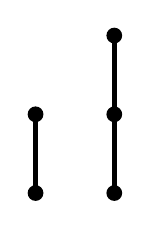
\begin{tikzpicture}
      \fill (0,0) circle (0.1);
      \fill (0,1) circle (0.1);
      \draw[ultra thick] (0,0)--(0,1);

      \fill (1,0) circle (0.1);
      \fill (1,1) circle (0.1);
      \fill (1,2) circle (0.1);
      \draw[ultra thick] (1,0)--(1,2);
    \end{tikzpicture}
    \hspace{2cm}
    
\begin{tikzpicture}
      \fill (0,0) circle (0.1);
      \fill (0,1) circle (0.1);
      \draw[ultra thick] (0,0)--(0,1);

      \fill (1,0) circle (0.1);
      \fill (1,1) circle (0.1);
      \draw[ultra thick] (1,0)--(1,1);

      \fill (1/2,2) circle (0.1);
      \draw[ultra thick] (1,1)--(1/2,2)--(0,1);
    \end{tikzpicture}
    \hspace{2cm}
    
\begin{tikzpicture}
      \fill (0,0) circle (0.1);
      \fill (0,1) circle (0.1);
      \draw[ultra thick] (0,0)--(0,1);

      \fill (3/2,0) circle (0.1);
      \fill (1,1) circle (0.1);
      \draw[ultra thick] (3/2,0)--(1,1);
      \fill (2,1) circle (0.1);
      \draw[ultra thick] (3/2,0)--(2,1);
    \end{tikzpicture}
  \]
  In the first case, $J(P) = [3] \times [4]$, so this works.
  \\
  In the second case, $J(P)$ has only two ideals with three elements, so this
  doesn't work.
  \\
  In the third case, $J(P)$, has four ideals of with two elements, so this
  doesn't work.
  \\~\\
  Thus $P = [2] + [3]$.
\end{solution}
\pagebreak
% -----------------------------------------------------
% Second problem
% -----------------------------------------------------
\begin{problem}{46 a} $[2]$ \\
  Let $f(n)$ be the number of sublattices of rank $n$ of the boolean algebra
  $B_n$. Show that $f(n)$ is also the number of partial orders $P$ on $[n]$.
\end{problem}

\begin{solution} \text{} \\
  Since $B_n$ is a distributive lattice, all rank $n$ sublattices of $B_n$ must
  also be distributive lattices. Thus each sublattice of $L \subset B_n$ can be
  written as $L \cong J(P)$ for some poset $P$, where $P$ is isomorphic to the
  set of join irreducibles of $L$. By proposition 3.4.5, since $L$ has rank $n$,
  $P$ must have $n$ elements. So every distributive lattices of rank $n$ gives
  a partial ordering of $[n]$.
  \\~\\
  This a bijection, because given some poset $P$, we can recover $L$ via $J$
  (namely, $L \cong J(P)$). Each distinct $P$ gives a distinct rank $n$
  sublattice of $B_n$ because
  (1) $J(P)$ is a distributive lattice,
  (2) $J(P)$ contains the ideal $[n]$,
  (and no larger ideal) and,
  (3) $J(P)$ includes the ideal $\emptyset$.
  % Let $\phi$ be a map which sends a poset $P$ (with underlying set $[n]$) to
  % $J(P) \subset B_n$.
  % Since $B_n$ is a finite distributive lattice, and every sublattice of a
  % finite distributive lattice is a finite distributive lattice, we can
  % take the set of join irreducibles of any rank $n$ sublattice, and this will
  % be isomorphic to a poset on $[n]$.
\end{solution}
\pagebreak
% -----------------------------------------------------
% Third problem
% -----------------------------------------------------
\begin{problem}{53} $[2]$ \\
  Let $P$ be a finite $n$-element poset. Simplify the two sums \[
    f(P) = \sum_{I \subset J(P)} e(I)e(\overline I),
  \] \[
    g(P) = \sum_{I \subset J(P)} \binom{n}{\#I} e(I)e(\overline I),
  \] where $\overline I$ denotes the complement $P - I$ of the order ideal $I$.
\end{problem}

\begin{proof}
\end{proof}
\pagebreak
% -----------------------------------------------------
% Fourth problem
% -----------------------------------------------------
\begin{problem}{57} ~
  \begin{enumerate}[a.]
    \item $[2]$ Let $P$ be an $n$-element poset. If $t \in P$, then set
    $\lambda_t = \#\{s \in P : s \leq t\}$.
    Show that \[
      e(P) \geq \frac{n!}{ \prod_{t \in P} \lambda_t}.
    \]
    \item $[2+]$ Show that the equality holds if and only if every component of $P$ is
    a rooted tree.
  \end{enumerate}
\end{problem}

\begin{proof}
  \begin{enumerate}[a.]
    \item By induction, the base case is clear. When $n=1$, there is only
    one poset with one linear extension. \[
      e([1]) = \frac{1!}{\lambda_{1}} \geq 1.
    \]
    Thus given some poset $P$, we can take the subposet $P - m$ (where $m$ is
    any maximal element in $P$) which is a disjoint union of posets
    $P_1 + P_2 + \hdots + P_k$ with $n_1, n_2, \hdots, n_k$ elements respectively.
    We have several choices of labels for $m$, but if we choose one of those
    arbitrarily, then we can choose the $n_i$ labels for $P_i$ and each can be
    permuted in $e(P_i)$ ways, so \begin{align*}
      e(P) &\geq \binom{n - 1}{n_1, n_2, \hdots, n_k}e(P_1)e(P_2)\hdots e(P_k) \\
      &\geq \frac{(n - 1)!}{n_1! n_2! \hdots n_k!} \cdot
      \frac{n_1!}{\prod_{t \in P_1} \lambda_t}\cdot
      \frac{n_2!}{\prod_{t \in P_2} \lambda_t}
      \cdots
      \frac{n_k!}{\prod_{t \in P_k} \lambda_t} \\
      &= ...
    \end{align*}
    (I was unable to finish this part, but I think the second part is right.)
    %
    \item By induction, the base case is clear. When $n=1$, there is only
    one poset (which is a rooted tree) with one linear extension. \[
      e([1]) = \frac{1!}{\lambda_{1}} = 1.
    \]
    Thus given some rooted tree $P$, we can take the subposet $P - \hat 1$, which
    is a disjoint union of rooted trees
    $P_1 + P_2 + \hdots + P_k$ with $n_1, n_2, \hdots, n_k$ elements respectively.
    Since $P$ has a unique maximum, it must be labeled with $n$, then we can
    then choose which letters go in each sub-tree (using a multinomial
    coefficient), and then there are $e(P_i)$ ways to order the $n_i$ labels
    for each $P_i$. Therefore \begin{align*}
        e(P) &= \binom{n - 1}{n_1, n_2, \hdots, n_k}e(P_1)e(P_2)\hdots e(P_k)
        \\
        &= \binom{n - 1}{n_1, n_2, \hdots, n_k}
        \frac{n_1!}{\prod_{t \in P_1} \lambda_t}
        \frac{n_2!}{\prod_{t \in P_2} \lambda_t}
        \hdots
        \frac{n_k!}{\prod_{t \in P_k} \lambda_t}
        \\
        &= \left(\frac{(n - 1)!}{n_1! n_2! \hdots n_k!}\right)
        \frac{n_1!n_2!\hdots n_k!}{\prod_{t \in P - \hat 1} \lambda_t}
        \\
        &= \frac{(n-1)!}{\prod_{t \in P - \hat 1} \lambda_t}
    \end{align*}
    Since all $n$ elements of $P$ are less than or equal to $\hat 1$,
    $\lambda_{\hat 1} = n$, \[
      n\prod_{t \in P - \hat 1} \lambda_t = \prod_{t \in P} \lambda_t
    \] and thus \[
      e(P) = \frac{n(n-1)!}{n\prod_{t \in P - \hat 1} \lambda_t} = \frac{n!}{\prod_{t \in P} \lambda_t}
    \] as desired.
  \end{enumerate}
\end{proof}
\end{document}
